\chapter[SCP-134 星眼孩童]{
    SCP-134 Star-Eyed Child\\
    SCP-134 星眼孩童
}

\label{chap:SCP-134}

\begin{figure}[H]
    \centering
    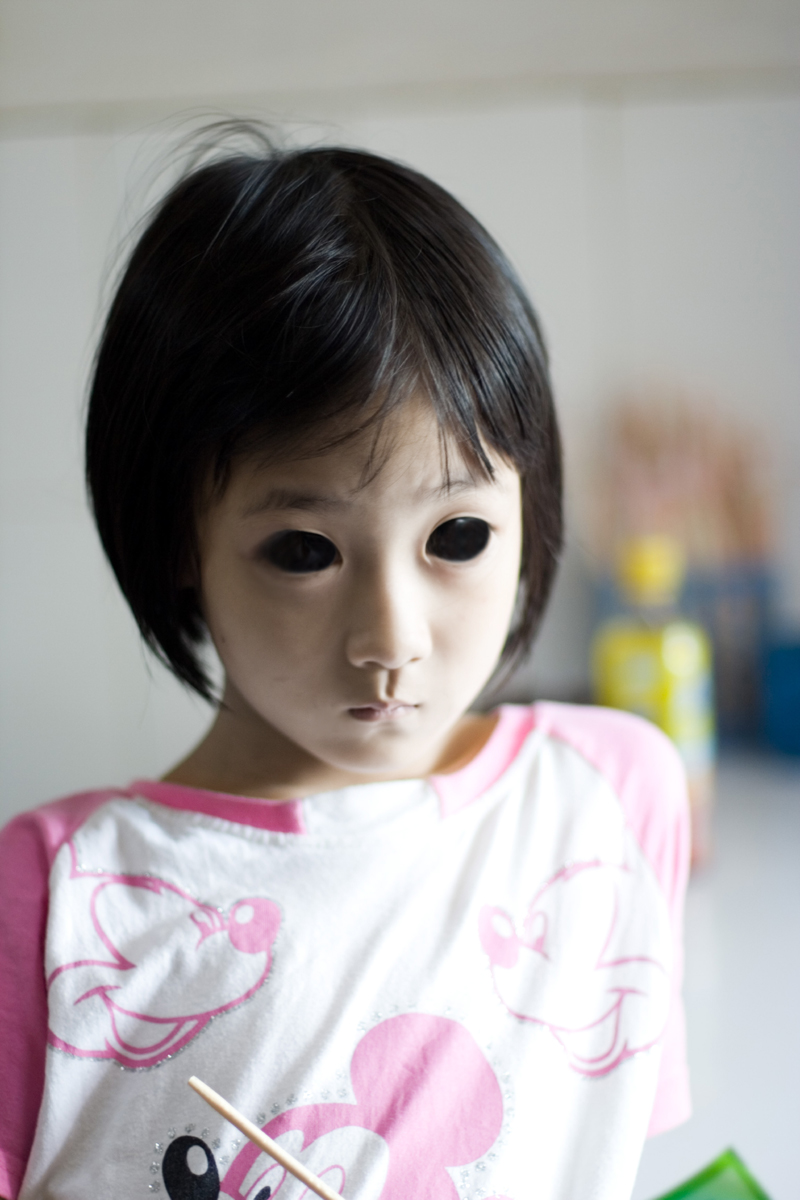
\includegraphics[width=0.5\linewidth]{images/SCP.134.jpg}
    \caption*{SCP-134,在普通亮度下}
\end{figure}

\bb{项目编号:}SCP-134

\bb{项目等级:}Safe

\bb{特殊收容措施:}SCP-134目前居住于一个尺寸为六乘八米,经过特殊布置的人型生物保管隔间内。因为SCP-134完全失明,房间内的家具必须配备特殊安全措施。SCP-134已经相当习惯于房间内所有物体的位置,并且基本通过记忆来辨认方向。任何为了“找乐子”而移动家具的人员都会被调至其他项目。SCP-134的房间目前包括:

一张带床垫的单人床。\\
一套粉色的床上用品,包括床单,被子和印有“Hello Kitty”图案的枕头。(注:尽管失明,SCP-134可以感觉到印刷图案并且显示出了对这种图案的偏好。)\\
一个衣橱和一个带抽屉的柜子,内含超小号儿童衣物。所有的抽屉都带有盲文及凸出印刷的英文标签。\\
一套玩偶之家玩具,包括玩偶和内部陈设。\\
八只填充动物玩具(三只猫,两只狗,一只长颈鹿,一只海豚以及一只熊猫)\\
一套儿童盲文读物。\\
一把椅子和一张桌子。\\
一套手工艺台,包括玩具黏土和积木。

SCP-134可能会要求的任何其他东西都必须先经过一个拥有3级以上权限的工作人员许可。如果房间内添置了任何东西,必须提前通知SCP-134的照看者以使SCP-134对环境中的新要素做好准备。SCP-134应定期受到与其年龄水平相符的基础教育和盲文教学。

\bb{描述:}SCP-134是一个█到█岁之间的亚洲女孩,黑色短发,体型单薄。对象在很多方面都表现正常并且拥有一个人类儿童的一切生理需要(食物,睡眠等)。然而SCP-134的眼部是两个黑洞,覆盖着一层外观与人类眼角膜相似的透明薄膜;眼科测试显示这层薄膜的弹性是普通人类眼角膜的150到200倍。SCP-134没有眼睑所以不会眨眼,也不能通过此黑色区域视物。对SCP-134的眼球后方的检查失败了,因为没有发现视网膜。在普通光照条件下,它们呈现为漆黑,但是在黑暗中,在其中可以看到非常暗淡的光芒。进一步的长时间曝光摄影和光放大测试表明光芒实际上来自星球和星系,清晰可见,似乎通过SCP-134的眼眶可以一定程度地望向深空。基金会天文学家Dr. ███████的研究正在进行中,但是时至今日没有识别出任何天体。

\begin{figure}[H]
    \centering
    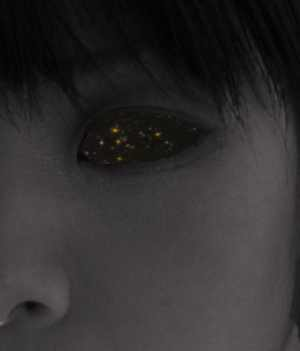
\includegraphics[width=0.35\linewidth]{images/SCP.134.2.jpg}
    \caption*{低亮度摄影中SCP-134的眼睛}
\end{figure}

声纳测试在SCP-134的颅骨内没有发现异常空腔;但是{[}数据删除]证明了确实存在{[}数据删除],眼眶是本地终端而星际空间是远程终端。视差测量表明远程终端的距离约二十到两千米远,并且以光速的二十倍到四十倍的速度移动;这种情况与SCP-134的位置,动作或新陈代谢没有任何联系。

光谱分析显示远程终端周期性地{[}数据删除]新位置;原因目前未知。变化的最短间隔是六天,最长间隔是五个星期。截止目前没有观察到过进行中的转移。

SCP-134没有显示出任何有敌意的行为,而且似乎对自己不自然的状况一无所知。SCP-134显现了与患有高度自闭症的儿童相似的症状,包括固定的行为模式和对变化的抵触。针对这点,为SCP-134配备了一位儿童教育专家以解决这些问题;专家提出适当的儿童教育需要一个私人名称,并且昵称SCP-134为“Stella”。SCP-134已经掌握了被以SCP编号称呼和进行身体测试之间的联系,并且在之前称呼她“Stella”的人以编号称呼她时表现出沮丧和消极合作。因此,不建议人员以她的名字称呼她除非想把与SCP-134之间的互动限制在谈话层面。

专家随后被解雇,因其对于被分配给他的SCP产生了过于亲近的兴趣。任何被发现称呼SCP-134为‘Stella’的人员都会被严厉训斥。

当被问及她的眼睛时,SCP-134声称对于其畸形没有任何认知,即使是在被允许感受正常的人类眼睛作为比较之后。

目前SCP-134没有自愿提供任何关于父母和身份的信息,尽管在被基金会寻获时SCP-134被称为“████”。SCP-134被证明温顺合作,因此工作人员必须显示出像对待其他客人一样的正常礼貌。基金会基于一份关于一个畸形儿被遗弃在日本横滨███████的███████████孤儿院的报告找到了SCP-134,在20██年将其置于监护之下,那时孤儿院的工作人员声称SCP-134█岁。从那以后SCP-134学会了英文口语,以及已经掌握的日语,并且展示了对盲文的熟悉,而对她的教育还在继续。
